\section{Overview} \label{sec:overview}

\subsection{Hybrid Recommender Architecture} \label{sec:hybrid-recommender-architecture}

From a high-level perspective, the \emph{readnext} framework comprises three main components: the Citation Recommender, the Language Recommender, and the Hybrid Recommender.
For consistent notation throughout this thesis, the term \emph{Hybrid Recommender} is capitalized when referring to the specific hybrid system developed in this thesis. Conversely, the lowercase version is used when referring to the general concept of hybrid recommender systems.


\subsubsection*{Citation Recommender}

The Citation Recommender generates recommendations based on five features of two different categories: three global document characteristics and two citation-based features.


\subsubsection*{Global Document Characteristics}

The global document characteristics are derived from a paper's metadata. The Citation Recommender uses the following three features:

\begin{itemize}
    \item The \emph{publication date} of the paper serves as an indicator of \emph{novelty}. More recent publications are given a higher score because they build on previous papers, compare and contrast their findings with existing results, and are thus perceived as more valuable. The publication date feature compensates for the lower citation count newer papers might encounter.
    \item The \emph{paper citation count} acts as a measure of \emph{document popularity}. Papers with higher citation counts are, on average and without any prior knowledge, considered more valuable and relevant.
    \item The \emph{author citation count} across all publications functions as a measure of \emph{author popularity}. Authors with a higher citation count are regarded as more influential in the research community. For papers with multiple authors, the citation count of the most-cited author is selected. This method is preferred over using the average citation count of all co-authors based on the assumption that the co-authorship of a single, well-established researcher has a more significant impact on the paper's reputation than the co-authorship of several less established researchers. Additionally, the value should be independent of the number of authors, which means aggregation measures like the sum of all co-author citation counts are not suitable.
\end{itemize}

These features are independent of the query paper for which recommendations are generated. For instance, the candidate paper with the highest citation count will always rank first among all candidates for that feature, irrespective of the specific query paper being considered.


\subsubsection*{Citation-based Features}

In addition to global document features, the Citation Recommender uses \emph{co-citation analysis} \cite{SmallCocitationScientific1973,Marshakova-ShaikevichSystemDocument1973} and \emph{bibliographic coupling} \cite{KesslerBibliographicCoupling1963} scores between the query paper and each candidate paper.
These are static citation analysis measures that neither consider the citation location nor the context.
While location-aware methods, such as \ac{CPA} \cite{GippCitationProximity2009} and section-based bibliographic coupling \cite{HabibSectionsbasedBibliographic2019}, often yield superior results, they necessitate full-text access to discern the location of citations.
As the full document texts are not available for this thesis, we stick to static citation analysis measures.

Unlike the global document characteristics, the citation-based features strongly depend on the query paper as they generate pairwise scores between the query paper and each candidate paper. As such, a particular candidate paper might have a high co-citation analysis score with one query paper but a low score with another.


\subsubsection{Language Recommender}

The Language Recommender employs the text content of the paper to generate recommendations.
Due to the lack of full text access, the recommender utilizes paper abstracts, which are first tokenized and then embedded into a vector space using one of eight language models.
Finally, the content similarity between query and candidate papers is calculated using the cosine similarity between their respective vector embeddings.

The eight language models can be categorized as follows: Keyword-based language models generating sparse vector embeddings and language models generating dense vector embeddings.
Dense vector embedding models are further divided into static and contextual embedding models.
Within each category, a popular foundational model (TF-IDF \cite{SaltonTermWeighting1987}, Word2Vec \cite{MikolovEfficientEstimation2013}, and BERT \cite{DevlinBERTPretraining2019}) is employed, as well as one or two variations developed to improve upon this base model (BM25 \cite{RobertsonOkapiTREC31995}, FastText \cite{BojanowskiEnrichingWord2017} \& GloVe \cite{PenningtonGloveGlobal2014}, and SciBERT \cite{BeltagySciBERTPretrained2019} \& Longformer \cite{BeltagyLongformerLongDocument2020}).


\subsubsection{Hybrid Recommender}

The Hybrid Recommender merges the recommendations of the Citation Recommender and the Language Recommender using the sequential cascade strategy (\Cref{sec:hybridization-techniques}).
Each recommender produces a preliminary list of 20 recommendation candidates, which the other recommender then re-ranks to generate the final ranking.
The value $n=20$ for the size of the candidate list is configurable by the user, but indicated a good trade-off between performance and computational complexity in our experiments.

If the Citation Recommender operates first, it ranks all candidate papers based on a weighted score from global document characteristics and citation-based features. The top 20 papers with the best weighted score are subsequently passed to the Language Recommender, which then re-ranks the candidate list based on content similarity of the paper abstracts.

\Cref{fig:hybrid-recommender} illustrates the interaction between the Citation Recommender and the Language Recommender within the hybrid system.

\begin{figure}[htb!]
    \centering
    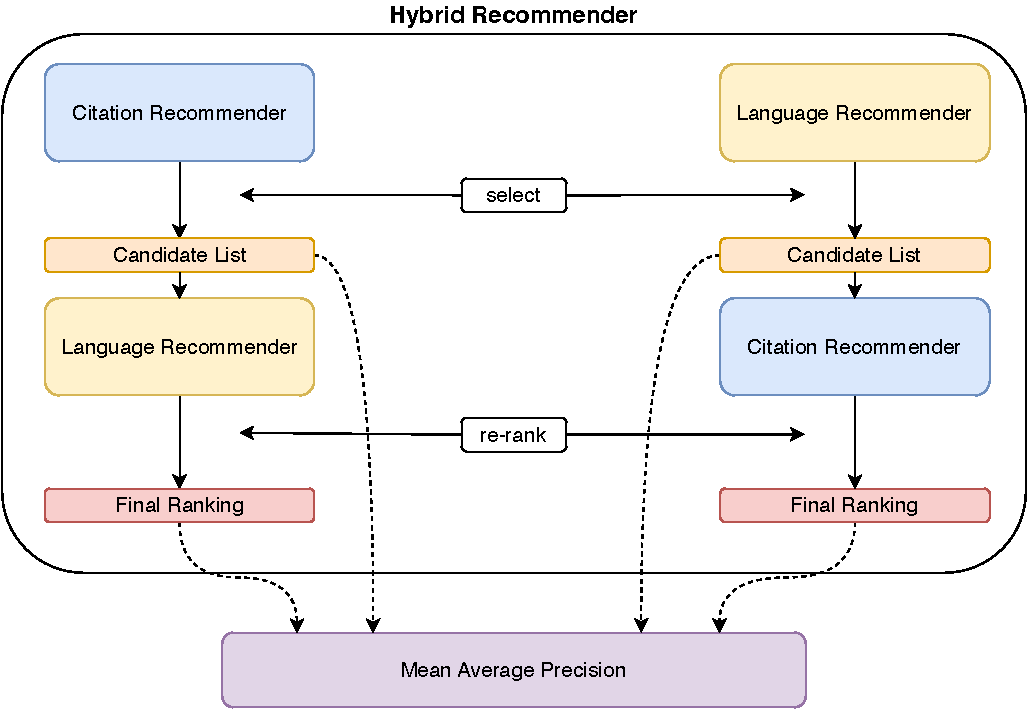
\includegraphics[width=0.9\textwidth]{diagrams/hybrid-recommender.pdf}
    \caption[Hybrid Recommender]{Hybrid Recommender Architecture. The Hybrid Recommender combines the recommendations of the Citation Recommender and the Language Recommender using a cascade strategy: Each recommender selects a candidate list of recommendations which is then re-ranked by the other recommender. The \ac{MAP} is calculated and compared for both candidate and both final rankings.}
    \label{fig:hybrid-recommender}
\end{figure}


\subsubsection{Evaluation}

Among the various metrics available for recommender systems (\Cref{sec:evaluation-of-recommender-systems}), the \ac{MAP} is selected as the primary evaluation metric for this thesis for the following reasons:

\begin{enumerate}
    \item \ac{MAP} considers the order of recommendations, emphasizing not just the relevance of the items but also their positioning early in the list \cite{TaifiMRRVs2020,RinkMeanAverage2023}. This is not the case for the Precision, Recall, and F1-Score metrics \cite{BaiScientificPaper2020}.
    \item All items on the recommendation list are considered, i.e. it's not only important to recommend relevant items but also to avoid irrelevant items. This is not the case for the \ac{MRR} metric, which only considers the first relevant item on the recommendation list \cite{SilveiraHowGood2019}.
    \item \ac{MAP} works with binary 0/1 encoded labels, which in this thesis indicate irrelevant/relevant recommendations. This is not the case for the \ac{NDCG} metric, which works better with graded relevance labels like irrelevant, somewhat relevant, relevant, and highly relevant \cite{SilveiraHowGood2019}.
\end{enumerate}

During the evaluation process, the \ac{MAP} is calculated not only for the final rankings of the Hybrid Recommender for both the \ac{C2L} and \ac{L2C} orderings, but also for both intermediate candidate lists.
Employing the same metric for both candidate and final rankings facilitates direct performance comparison. This includes: (i) contrasting the candidate lists of the Citation Recommender and the Language Recommender to identify the superior candidate selector, (ii) evaluating final recommendation rankings to pinpoint the optimal hybrid ordering, and (iii) comparing candidate and final rankings to assess if the re-ranking step enhances recommendation quality.
